\documentclass[11pt]{article}
\usepackage[margin=0.85in]{geometry}
\usepackage[T1]{fontenc}
% newtx not in this TeX Live; use Computer Modern\n\usepackage{lmodern}
% \usepackage{microtype}
\usepackage{amsmath,amssymb,bm}
\usepackage{booktabs,longtable,tabularx,array,multirow}
\usepackage{enumitem}
\usepackage{graphicx}
\usepackage{tikz}
\usetikzlibrary{arrows.meta,positioning,shapes.geometric,fit}
\usepackage[authoryear,round]{natbib}
\usepackage{xcolor}
\usepackage{hyperref}
\usepackage{xurl}
\usepackage{fancyhdr}
\usepackage{caption}
\hypersetup{hidelinks,pdfauthor={Rajeev Yadav, Ph.D.},pdftitle={FinCompass: Bayesian Probabilistic Forecasting with Evidence-Tiered Validation and Governed Live Adaptation}}
\setlength{\parindent}{1.1em}
\setlength{\parskip}{0.25em}
\setlength{\emergencystretch}{2em}
\newcommand{\Prb}{\mathbb{P}}
\newcommand{\E}{\mathbb{E}}
\newcommand{\I}{\mathbb{I}}
\newcommand{\sigmoid}{\operatorname{sigmoid}}
\newcommand{\logit}{\operatorname{logit}}
\newcommand{\FC}{\textsc{FinCompass}}
\pagestyle{fancy}
\fancyhf{}
\fancyhead[L]{\small FinCompass Technical Manuscript}
\fancyhead[R]{\small Rajeev Yadav, Ph.D.}
\fancyfoot[C]{\thepage}
\title{\textbf{FinCompass: Bayesian Probabilistic Forecasting with Evidence-Tiered Validation and Governed Live Adaptation}}
\author{Rajeev Yadav, Ph.D.\\\texttt{rajeevyadav@gmail.com}}
\date{August 2026}
\begin{document}
\maketitle

\begin{abstract}
Anyone who has shipped a forecasting tool has felt this tension. If every fitted model is accepted, the system risks presenting unstable scores as probabilities. If every model that misses a demanding predictive-skill threshold is discarded, the user may be left with no forecast even when a coherent, leakage-controlled, calibrated Bayesian model exists. This paper lays out a layered design that keeps four questions apart: whether the data and computation are valid, whether a probability model is estimable, whether stronger out-of-sample predictive evidence has been demonstrated, and whether the data provenance supports stronger market-grade claims. The implementation combines a regularized Bayesian logistic reference model, an experimental regime-aware Bayesian extension, a stronger nonlinear ensemble, explicit applicability contracts, purged chronological validation, calibration, proper scoring rules, block-bootstrap uncertainty, walk-forward stability, model freshness, immutable retraining candidates, explicit replacement, and a separately governed Live residual. The system also contains a provider-independent analytical layer for performance, risk, normalized statements, ratios, valuation, fixed income, options, portfolio analytics, factors and technical indicators. The analytical layer is deliberately kept separate from the forecasting feature set unless a feature is explicitly registered, point-in-time reviewed, trained and validated. Reference results are reported to demonstrate the software and governance framework rather than to claim durable alpha. The paper closes with implementation failure modes, acceptance criteria for new-ticker forecasting, and the distinction between a statistically usable probability, demonstrated predictive skill, and a trading recommendation.
\end{abstract}

\noindent\textbf{Keywords:} Bayesian forecasting; probability calibration; Brier score; temporal validation; hidden Markov model; model governance; online learning; point-in-time data; financial analytics.

\paragraph{How to Read This Paper.}
The first half is the product argument: what a usable forecast is, what event is being estimated, and why validity, skill and market-grade evidence are different questions. The middle is the model stack and the validation contract. The last third is operational: freshness, retraining, Live adaptation, analytics that must not leak into the model, and the acceptance tests a reviewer can actually run. Tables in the results section are reference evidence for the software, not a claim that the bundled sample predicts markets in general.

\section{Introduction}
The first product question is deceptively simple: when is a model \emph{usable}? In many software systems the answer is implicitly binary. A model is trained, a validation gate is evaluated, and the model either passes or disappears. That binary is convenient for software. It is a poor scientific contract, because it folds several different questions into one switch.

A model can be invalid because the target leaks future information, because the chronological split is broken, because the optimizer does not converge, because the posterior covariance is non-finite, because the model is applied to an unsupported market, or because the probability output cannot be reconstructed from the declared features. Those are hard failures. They should block a forecast.

A different situation occurs when the construction is valid but the model does not materially improve on an unconditional reference forecast. In that case the correct conclusion is not automatically ``the model does not exist.'' The more defensible conclusion is that the probability estimate has limited demonstrated predictive evidence. The system may still expose it as a baseline, provided that the limitation is explicit and stronger model tiers remain subject to stronger gates.

The architecture follows from that distinction. The central principle is
\begin{equation}
\text{model validity}\neq\text{predictive skill}\neq\text{market-grade evidence}.
\end{equation}
The practical consequence is a model ladder rather than a single pass/fail state. The ladder begins with a simple reference probability, progresses through a regularized Bayesian model and a regime-aware research extension, and permits stronger nonlinear models only when they demonstrate incremental value under a protected temporal evaluation protocol.

\section{Product Boundary and Analytical Planes}
\FC\ is organized into three deliberately separated analytical planes plus a deterministic analytics library.

\begin{figure}[ht]
\centering
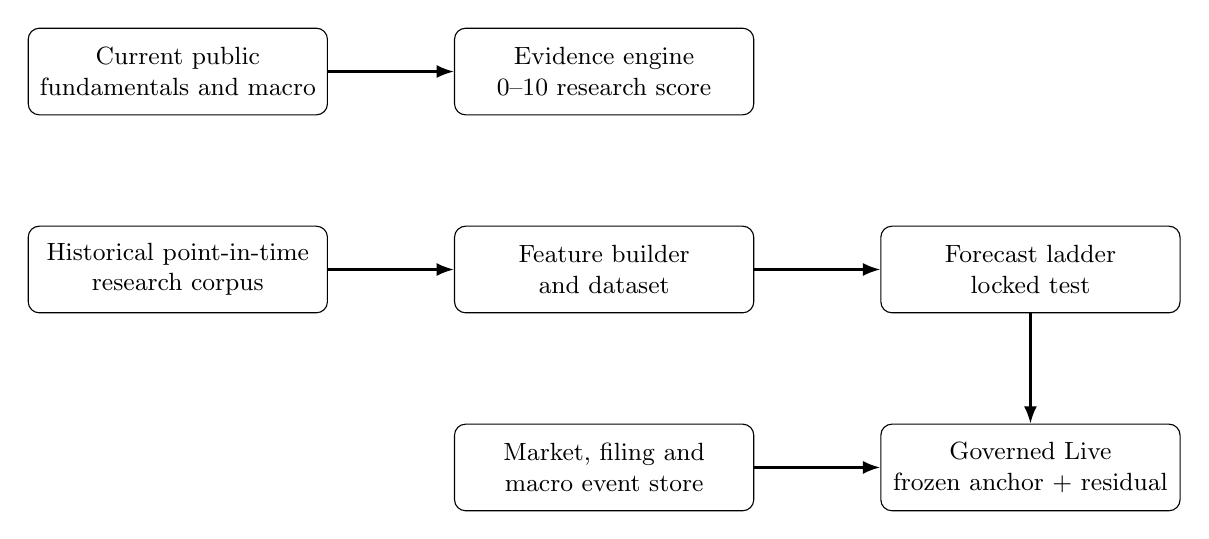
\begin{tikzpicture}[
  font=\small,
  box/.style={draw,rounded corners,align=center,minimum width=38mm,minimum height=11mm,inner sep=3pt},
  arr/.style={-{Latex[length=2.2mm]},thick}
]
\node[box] (current) {Current public\\fundamentals and macro};
\node[box, right=16mm of current] (evidence) {Evidence engine\\0--10 research score};
\node[box, below=14mm of current] (hist) {Historical point-in-time\\research corpus};
\node[box, right=16mm of hist] (features) {Feature builder\\and dataset};
\node[box, right=16mm of features] (anchor) {Forecast ladder\\locked test};
\node[box, below=14mm of features] (events) {Market, filing and\\macro event store};
\node[box, right=16mm of events] (live) {Governed Live\\frozen anchor + residual};
\draw[arr] (current)--(evidence);
\draw[arr] (hist)--(features);
\draw[arr] (features)--(anchor);
\draw[arr] (anchor)--(live);
\draw[arr] (events)--(live);
\end{tikzpicture}
\caption{Four planes stay separate: current evidence scoring, historical forecasting, governed Live, and (not drawn) deterministic analytics. Analytics never become Forecast features unless a versioned contract admits them.}
\end{figure}

The evidence engine summarizes currently observed information across Quality, Financial Durability, Safety, Valuation and Cycle. Its posterior is about an evidence score, not a future return. The forecast plane estimates the probability of a precisely defined forward event. The Live plane begins from a frozen forecast anchor and may apply a bounded residual only after a separate sequential validation gate becomes active. A fourth library provides deterministic analytics that are useful for interpretation but remain outside the model unless explicitly admitted through a feature-governance process.

The split is not a slide-deck convenience. It prevents a common category error: treating every available analytical metric as a predictor. A DCF value, a Sharpe ratio, a technical indicator and a forecast probability answer different questions and have different data requirements.

\section{Forecast Target and Event Semantics}
Let $i$ index an instrument, $b$ a benchmark, $t$ the observation date, and $H$ the forecast horizon. Let $\tau_H(t)$ denote the exact horizon endpoint under the declared session convention. Define forward returns
\begin{align}
R_{i,t}^{(H)} &= \frac{P_i(\tau_H(t))}{P_i(t)}-1,\\
R_{b,t}^{(H)} &= \frac{P_b(\tau_H(t))}{P_b(t)}-1.
\end{align}
For hurdle $\eta$, the event is
\begin{equation}
Y_{i,t}^{(H,\eta)}=\I\left[R_{i,t}^{(H)}-R_{b,t}^{(H)}>\eta\right].
\end{equation}
The forecast is
\begin{equation}
p_{i,t}=\Prb\left(Y_{i,t}^{(H,\eta)}=1\mid\mathcal{F}_t\right),
\end{equation}
where $\mathcal{F}_t$ contains only information observable by time $t$.

Three details are essential.

\paragraph{Benchmark Dependence.} The probability is benchmark-relative. A 60\% probability of outperforming the S\&P 500 is not equivalent to a 60\% probability of a positive absolute return.

\paragraph{Horizon Dependence.} A six-month model and a twelve-month model estimate different events. One cannot substitute for the other merely because both are trained on the same security.

\paragraph{Label Maturity.} A row observed at time $t$ has no supervised label until the exact endpoint $\tau_H(t)$ exists. A data refresh may create new features immediately, but it cannot manufacture a future outcome before the horizon matures. This distinction is central to both offline retraining and Live adaptation.

\section{Applicability as Part of the Scientific Contract}
Computational compatibility is not the same as scientific applicability. A model can calculate features for an instrument and still be inappropriate for that instrument. Every forecast artifact therefore declares an applicability domain including, at minimum:
\begin{itemize}[itemsep=0.2em]
\item asset class;
\item region or market;
\item security type;
\item benchmark family;
\item feature frequency;
\item horizon;
\item training period and training universe type;
\item feature contract and data-basis assumptions.
\end{itemize}

The resolver first classifies the instrument, then chooses a benchmark policy, then searches only model families that match the declared domain. This design enables pooled family models without pretending that one universal model applies to every market. A newly entered US common stock can use a pooled US-equity family model even if the ticker was not itself in the original training set, but a Canadian equity, bond ETF, commodity proxy or cryptoasset must not silently inherit that model.

\section{Data Architecture and Provenance}
\subsection{Durable Local Research Store}
The forecasting pipeline uses a durable local research corpus that is separate from the current-data cache used by the evidence workspace. Acquisition and training are separate operations. Training never downloads data implicitly. This makes experiments reproducible and allows the user to inspect exactly what corpus was used.

The update pattern is incremental:
\begin{enumerate}[itemsep=0.2em]
\item determine the last retained observation;
\item request a short overlap plus the missing tail;
\item compare overlap values;
\item journal provider revisions;
\item append new observations;
\item rebuild one symbol if a price-basis conflict is detected;
\item preserve raw provider frames and hashes for audit.
\end{enumerate}

The accumulated corpus is used for retraining. The delta alone is never treated as the full training set.

\subsection{Point-in-Time Fundamentals}
A financial statement value becomes usable only when it was public. For SEC-derived features, filing availability dates are therefore more important than fiscal period-end dates. The as-of merge must use the filing timestamp so that a December year-end result filed in February is not available to a January forecast. This is a standard source of look-ahead bias in financial backtests.

\subsection{Price-Basis Consistency}
Mixing raw and adjusted prices can create artificial returns. The research store records the price basis and treats an overlap conflict as a data integrity event. If a symbol changes basis, the safe response is to rebuild that symbol on one coherent basis rather than append incompatible observations.

\section{Feature Construction}
The reference forecasting features are deliberately compact. The exact contract is versioned. A typical monthly relative-return contract includes:
\begin{itemize}[itemsep=0.15em]
\item relative returns over multiple lookbacks;
\item absolute and benchmark volatility;
\item rolling drawdown;
\item distance from a moving trend or trailing high;
\item relative trend measures;
\item momentum acceleration;
\item downside volatility;
\item benchmark correlation and rolling beta;
\item optional regime-state probabilities.
\end{itemize}

All price features are backward-looking. The forward shift is confined to target construction. This permits a direct leakage test: perturbing prices after $t$ must not alter features at or before $t$.

The feature policy intentionally rejects the idea that hundreds of available analytics should automatically enter the model. Feature proliferation increases search degrees of freedom and therefore the risk of backtest overfitting \citep{white2000reality,harvey2016crosssection,bailey2017pbo}. A deterministic metric becomes a model feature only after it receives a versioned definition, point-in-time review, missing-data policy, experiment record and proper temporal validation.

\section{Bayesian Reference Model}
For standardized feature vector $x$, the reference model is
\begin{equation}
\Prb(Y=1\mid x,\beta)=\sigmoid(\beta_0+x^\top\beta).
\end{equation}
Slope coefficients receive Gaussian shrinkage priors,
\begin{equation}
\beta_j\sim\mathcal{N}(0,\tau^2),
\end{equation}
with a wider prior for the intercept. The implementation estimates the posterior mode and uses a Laplace approximation for the posterior covariance. This yields an interpretable low-capacity model with explicit uncertainty and controlled regularization.

If $\hat\beta$ is the posterior mode and $\Sigma$ the Laplace covariance, posterior coefficient draws are approximated by
\begin{equation}
\beta^{(s)}\sim\mathcal{N}(\hat\beta,\Sigma),
\end{equation}
and propagated to predictive probabilities
\begin{equation}
p^{(s)}(x)=\sigmoid(\beta_0^{(s)}+x^\top\beta^{(s)}).
\end{equation}
Quantiles of $\{p^{(s)}\}$ provide a model-uncertainty interval. This interval is not a full predictive interval for realized returns; it is uncertainty in the model probability under the approximation.

\section{Calibration}
A logistic score is not guaranteed to be well calibrated in finite samples. Calibration is therefore a separate step fitted only on a later validation block. The locked test is untouched until feature construction, component fitting and calibration choices are complete.

For binary outcome $y$ and forecast $p$, the Brier score is
\begin{equation}
BS=(p-y)^2,
\end{equation}
and log loss is
\begin{equation}
LL=-\left[y\log p+(1-y)\log(1-p)\right].
\end{equation}
Both are proper scoring rules \citep{brier1950verification,gneiting2007proper}. Brier skill compares the model with a reference probability, usually the development-set event rate. Expected calibration error summarizes bin-level discrepancies, while calibration slope/intercept assess systematic over- or under-dispersion.

Calibration should not be treated as a cosmetic post-processing step. A model can rank observations reasonably well and still produce poor probabilities. Conversely, a low AUC model can be well calibrated but provide little discriminatory value. A probability system should report both dimensions.

\section{Regime-Aware Bayesian Model}
Financial relationships can vary across market environments. The regime-aware extension introduces a latent state $S_t$ estimated from benchmark-only, backward-looking features. A simple three-state Gaussian hidden Markov model is sufficient for the first research layer:
\begin{equation}
S_t\in\{1,2,3\},\qquad \Prb(S_t\mid S_{t-1})=A_{S_{t-1},S_t}.
\end{equation}
The emission vector may include benchmark one-month return, six-month return and six-month volatility. State labels are ordered after fitting for interpretability, for example risk-off, neutral and risk-on.

The forecast becomes
\begin{equation}
\Prb(Y=1\mid x,\pi_t)=\sigmoid(\beta_0+x^\top\beta+\gamma^\top\pi_t),
\end{equation}
where $\pi_t$ contains filtered state probabilities. Filtering, not smoothing, is used at evaluation time so future observations cannot rewrite earlier state probabilities.

The regime model is not automatically preferred. It is a candidate in the model ladder and must demonstrate incremental value. This is important because adding latent states increases flexibility and can degrade calibration even when it improves fit.

\section{Enhanced Nonlinear Model}
The enhanced model combines a Bayesian logistic component, histogram gradient boosting and a regularized random forest. Each component is calibrated on a dedicated chronological stage. Non-negative ensemble weights that sum to one are learned on a separate stacking stage, followed by a final calibration stage.

The validation region is therefore partitioned into distinct roles rather than reused repeatedly. The locked test never participates in feature selection, calibration choice, weight fitting or threshold tuning.

The enhanced model is evaluated against two references:
\begin{enumerate}[itemsep=0.2em]
\item the unconditional event-rate forecast;
\item the Bayesian reference model.
\end{enumerate}
A more complex model is retained only when the extra complexity is justified by more robust predictive evidence.

\section{Temporal Validation}
Random train/test splitting is inappropriate for overlapping long-horizon financial labels. The system uses chronological partitions with target-end purging and an embargo. Rows whose forward label crosses a later fitting boundary are removed from the earlier partition.

The locked test is a protected resource. Repeatedly changing features or hyperparameters in response to locked-test results turns the locked test into another validation set. The process therefore separates development from final evaluation and records the exact split dates and row counts.

\subsection{Walk-Forward Stability}
A single locked-test average can hide instability. Purged walk-forward evaluation checks whether the sign and magnitude of skill are reasonably persistent across later windows. The objective is not to guarantee future stability but to reject candidates whose apparent average performance is driven by one isolated period.

\subsection{Block Bootstrap}
Long-horizon labels overlap in time and same-date cross-sectional observations are correlated. The bootstrap therefore resamples blocks of observation dates while keeping the same-date cross-section together. This provides uncertainty bounds that are more conservative than an iid row bootstrap \citep{kunsch1989jackknife,politis1994stationary}.

\section{Validity Gates and Evidence Tiers}
The model state machine separates hard validity from stronger evidence.

\begin{longtable}{p{0.18\textwidth}p{0.42\textwidth}p{0.15\textwidth}p{0.15\textwidth}}
\toprule
State & Meaning & Forecast & Adaptive Live\\
\midrule
\endhead
Invalid & Data, chronology, numerical fit, feature contract or applicability is not scientifically coherent. & No & No\\
Bayesian baseline & Hard-valid probability model; stronger predictive skill not established. & Yes, Limited evidence & Tracking only\\
Validated research & Strong configured temporal and probability gates passed on the declared research corpus. & Yes & Eligible\\
Validated market & Research gate plus stronger historical-universe and point-in-time data controls. & Yes & Eligible\\
\bottomrule
\end{longtable}

Hard validity includes sufficient rows and both classes, valid chronology, matured labels, feature-contract integrity, benchmark alignment, finite parameters, finite posterior covariance, valid probabilities, calibration feasibility and applicability-domain match. Failure blocks the model.

Predictive evidence includes Brier skill, log-loss skill, AUC, ECE, calibration slope, bootstrap bounds, temporal breadth and walk-forward stability. Failure to meet the stronger gate does not automatically erase a hard-valid Bayesian baseline.

This distinction protects both usability and scientific honesty. It prevents the system from manufacturing a strong claim by weakening gates, while also preventing every weak-but-valid Bayesian model from being mislabeled as a software failure.

\section{Model Selection and the Model Ladder}
The default selection order is:
\begin{equation}
\text{validated market}\;>\;\text{validated research}\;>\;\text{Bayesian baseline}.
\end{equation}
Selection is restricted to the exact applicability domain and requested horizon. Regime-aware models can be exposed as research alternatives without being preferred in Guided use unless their evidence tier and contract justify it.

The model ladder is important operationally because the user should not have to train a bespoke model for every new supported ticker. The model family is pooled. New ticker data are needed to construct current features; they are not necessarily needed to retrain the family model before a first forecast can be produced.

\section{Freshness: Three Concepts, Not One}
A robust implementation must separate three freshness questions.

\subsection{Instrument-Data Freshness}
Can the current ticker and benchmark supply enough recent observations to construct today's features?

\subsection{Model-Training Freshness}
How old is the actual training corpus used to fit the pooled family model?

\subsection{Retrainability Freshness}
How many new eligible family observations and matured labels exist after the model's training cutoff?

These are not interchangeable. A newly entered ticker can have current data through 2026 while the family model was trained through 2022. The ticker's recency does not itself prove that a retrain is required before forecasting. A stale-but-hard-valid model can remain forecast-eligible with a warning while an update is recommended separately.

\section{Retraining and Immutable Candidates}
Retraining uses the accumulated local corpus. If $D_0$ is the historical corpus and $\Delta D$ the verified update,
\begin{equation}
D_{new}=D_0\cup \Delta D\cup D_{accepted\ revisions}.
\end{equation}
Only matured labels are admitted to supervised fitting.

A retrain never overwrites the current model. If $M_1$ is current and retraining produces $M_2$, then $M_2$ is a new immutable artifact with lineage pointing to $M_1$. The current model survives not-ready, failed, rejected and validated candidate states. Explicit replacement is a separate action. This prevents ``newest file wins'' behavior and preserves reproducibility.

A retraining contract should be explicit in the manifest. Display names and profile names are not training recipes. The contract should declare the trainer family, recipe ID, horizon, benchmark family, feature contract and whether runtime retraining is supported.

\section{Failure-Safe Guided Behavior}
The user-facing workflow should be resilient to model-maintenance failure. The correct logic is:
\begin{quote}
If a hard-valid applicable model exists, Forecast remains available. Model maintenance may be recommended, but an unsuccessful optional update must fall back to the current model rather than strand the user.
\end{quote}

This leads to a capability-oriented planner with fields such as \texttt{can\_forecast\_now}, \texttt{can\_start\_live\_now}, \texttt{model\_update\_available}, and \texttt{model\_update\_required}. A single maintenance action should not accidentally become a blocking prerequisite.

\section{Live Architecture}
\subsection{Frozen Anchor}
Live begins from the selected forecast probability $p_0$. The anchor is frozen for that forecast instance.

\subsection{Event Vector}
Fresh market, filing and macro context is transformed into a separately governed event vector $z_t$. The adaptive candidate is
\begin{equation}
\logit(p_{cand,t})=\logit(p_0)+\delta(z_t).
\end{equation}
The residual is bounded in log-odds space, and the final probability is clipped to configured limits.

\subsection{Delayed Learning}
Fresh events can change the candidate immediately, but model parameters update only after the original forward target matures. Each pending observation stores the ticker, benchmark, base model ID, settings fingerprint, observation date, entry prices, anchor probability, candidate probability, feature vector, horizon and hurdle.

When the exact horizon endpoint becomes available, the outcome is resolved using the H-th common trading session rather than whatever price happens to be latest at processing time. This preserves the original target definition.

\subsection{Prequential Gate}
Adaptive influence requires sufficient matured observations, sufficient unique observation dates, minimum elapsed span, date-balanced Brier/log-loss non-inferiority, acceptable calibration error, fresh sources and no active drift alert. Otherwise the applied residual is zero and the display falls back to the frozen anchor. This is a prequential predict-before-update design in the sense of \citet{dawid1984prequential}.

\subsection{Baseline Live Tracking}
A Bayesian baseline can be tracked in Live without activating adaptive learning. In that mode the current and original forecast are identical, the system monitors freshness, and no pending adaptive label is created. This gives the user a coherent Live workspace without implying that a weak-evidence model has earned adaptive control.

\section{Deterministic Analytics Library}
The analytical layer is provider-independent at the formula level. Providers or importers supply data; the kernel consumes canonical arrays or normalized statements. Each metric should expose a result envelope containing formula ID, period, as-of date, inputs, source references, quality flags and method version.

\subsection{Performance Analytics}
Examples include annualized geometric return, annualized volatility, Sharpe ratio, Sortino ratio, maximum drawdown, Calmar ratio, beta, tracking error and information ratio. These summarize historical behavior. They are not forecasts.

For periodic returns $r_t$, geometric annualized return at $m$ periods per year is
\begin{equation}
R_{ann}=\left(\prod_{t=1}^T(1+r_t)\right)^{m/T}-1.
\end{equation}
Annualized volatility is
\begin{equation}
\sigma_{ann}=s_r\sqrt{m}.
\end{equation}

\subsection{Risk Analytics}
Historical and Gaussian VaR, historical expected shortfall, EWMA volatility, drawdown magnitude and drawdown duration are included. VaR is explicitly a threshold under a stated method and confidence level; it is not the maximum possible loss.

\subsection{Technical Analytics}
Moving averages, EMA, RSI, MACD, Bollinger Bands, ATR and related trend/volatility summaries are computed from price/volume histories. Their existence does not imply predictive value.

\subsection{Normalized Statements and Ratios}
Provider vocabulary is mapped into canonical income-statement, balance-sheet and cash-flow fields. Missing accounting items remain missing rather than being silently converted to zero. Derived fields are flagged as derived. Ratios include profitability, liquidity, leverage, efficiency, cash-flow and per-share measures. Non-positive or missing denominators return unavailable results rather than misleading finite values.

\subsection{DCF Valuation}
The unlevered FCFF identity is
\begin{equation}
FCFF_t=EBIT_t(1-T_t)+D\&A_t-CapEx_t-\Delta NWC_t.
\end{equation}
Enterprise value is
\begin{equation}
EV=\sum_{t=1}^{N}\frac{FCFF_t}{(1+WACC)^t}+\frac{TV_N}{(1+WACC)^N}.
\end{equation}
The result is scenario dependent. Sensitivity to WACC, terminal growth and margin assumptions is therefore more informative than a single point estimate.

\subsection{Fixed Income}
The library includes bond present value, current yield, yield to maturity, Macaulay duration, modified duration, convexity and DV01. Inputs and compounding conventions are explicit.

\subsection{Options}
European Black-Scholes-Merton pricing with continuous dividend yield and Delta, Gamma, Vega, Theta and Rho are included, together with implied-volatility inversion. These are model identities under stated assumptions, not probabilities of profit.

\subsection{Portfolio Analytics}
Portfolio return, covariance, volatility and Euler risk contributions are derived from explicit weights and historical returns or a covariance matrix. Individual security forecast probabilities are not naively averaged into a portfolio probability.

\subsection{Factor Analytics}
OLS factor estimation provides coefficients, standard errors, t-statistics, $R^2$, adjusted $R^2$, residuals, CAPM-style alpha/beta, named factor loadings and rolling beta. Statistical significance is not automatically investment significance, and in-sample exposure is not a forward forecast.

\section{Evidence Score Versus Forecast Probability}
The evidence engine and forecast engine estimate different objects. The evidence score aggregates contemporaneous evidence into a posterior distribution over a 0--10 research score. The forecast model estimates a forward event probability. A statement such as $\Prb(\text{score}\ge 8)=0.70$ must not be interpreted as a 70\% probability of future outperformance.

This distinction is important in user interfaces because both outputs are percentages. The application should name the object explicitly whenever a probability is shown.

\section{Reference Implementation Results}
The bundled reference corpus contains monthly data for eight US equities and the S\&P 500 benchmark through June 2022. It is suitable for software and research demonstrations but does not establish market-grade historical-universe controls. The following results therefore demonstrate the evidence-tier framework, not durable alpha.

\begin{table}[ht]
\centering
\caption{Bayesian reference locked-test results.}
\begin{tabular}{rrrrrl}
\toprule
Horizon & Test $n$ & ROC AUC & Brier skill & ECE & Tier\\
\midrule
6 months  & 539 & 0.419 & -0.023 & 0.056 & Bayesian baseline\\
12 months & 532 & 0.480 & -0.012 & 0.035 & Bayesian baseline\\
24 months & 518 & 0.415 & -0.004 & 0.064 & Bayesian baseline\\
36 months & 497 & 0.303 & -0.108 & 0.199 & Bayesian baseline\\
\bottomrule
\end{tabular}
\end{table}

The twelve-month baseline is the clearest illustration of the tier concept. It is hard-valid and has low ECE on the locked sample, but its AUC is below 0.5 and its skill relative to the reference probability is slightly negative. It should not be promoted to validated research, yet the software can still expose it as a limited-evidence Bayesian reference estimate.

\begin{table}[ht]
\centering
\caption{Regime-aware Bayesian locked-test results.}
\begin{tabular}{rrrrrl}
\toprule
Horizon & Test $n$ & ROC AUC & Brier skill & ECE & Tier\\
\midrule
6 months  & 539 & 0.444 & -0.045 & 0.086 & Bayesian baseline\\
12 months & 532 & 0.508 & -0.059 & 0.067 & Bayesian baseline\\
24 months & 518 & 0.485 &  0.009 & 0.029 & Bayesian baseline\\
36 months & 497 & 0.321 & -0.043 & 0.163 & Bayesian baseline\\
\bottomrule
\end{tabular}
\end{table}

The 24-month regime model shows slightly positive proper-score skill in this sample, but the broader evidence contract does not justify promotion. The result illustrates why a model ladder should be comparative rather than complexity-driven.

The stronger twelve-month enhanced model achieved approximately ROC AUC 0.576, Brier skill 0.036, log-loss skill 0.027 and ECE 0.045 on its declared locked test, allowing a validated-research classification under the configured gate. These are modest research results, not claims of universal validity or deployable alpha.

\section{New-Ticker Acceptance Criterion}
A practical forecasting product must be evaluated on the path a normal user actually takes. The minimum acceptance criterion for a supported new US common-stock ticker is:
\begin{enumerate}[itemsep=0.2em]
\item classify the instrument;
\item resolve the benchmark family;
\item obtain or update local price history if necessary;
\item select the strongest applicable pooled model family;
\item produce a forecast without requiring bespoke per-ticker training;
\item start Live in either tracking-only or adaptive-eligible mode according to the selected tier;
\item preserve coherent state after restart.
\end{enumerate}

If an optional model update fails scientifically, the current hard-valid forecast should remain available. This is a product-level safety property. A unit test that merely verifies the presence of an ``Update model'' button is not evidence that the workflow works.

\section{Failure Modes and Defensive Behavior}
Important failure modes include:
\begin{longtable}{p{0.27\textwidth}p{0.31\textwidth}p{0.34\textwidth}}
\toprule
Failure & Scientific risk & Required behavior\\
\midrule
\endhead
Wrong benchmark family & Event meaning changes & Block or resolve correctly before forecasting\\
Mixed raw/adjusted prices & Artificial returns & Rebuild affected symbol on one basis\\
Immature labels & Future leakage & Exclude until exact endpoint exists\\
Random temporal split & Leakage and dependence distortion & Use chronological purge/embargo\\
Uncalibrated score shown as probability & Misleading confidence & Calibrate or label limitation explicitly\\
New ticker makes pooled model ``stale'' & Unnecessary retraining dead end & Separate ticker freshness from family-model freshness\\
Display profile used as training recipe & Update endpoint failure & Use explicit retraining contract\\
Baseline activation attempted for adaptive Live & Governance violation & Start tracking-only Live without activation\\
Optional update failure destroys current Forecast & Product dead end & Keep current model and restore Forecast\\
Repeated locked-test tuning & Backtest overfitting & Protect locked test and record experiments\\
\bottomrule
\end{longtable}

\section{Reproducibility and Artifact Governance}
Every model artifact should bind:
\begin{itemize}[itemsep=0.15em]
\item serialized model hash;
\item dataset manifest hash;
\item training, validation and test ranges;
\item target definition;
\item benchmark;
\item feature contract;
\item settings;
\item validation report;
\item applicability domain;
\item data-quality flags;
\item lineage and parent model where applicable;
\item explicit training contract for runtime retraining.
\end{itemize}

Activation is separate from validation. A validated candidate is not automatically production-selected. Explicit activation history makes model changes auditable and reversible.

\section{Interpretation Boundaries}
The system does not claim that a probability estimate is a recommendation, that a validated-research result is proof of alpha, that DCF is a target price, that VaR is the worst possible loss, that a factor loading is causal, or that a backtest result will persist.

The central communication rule is proportionality between evidence and claim strength. A limited-evidence baseline should be useful without being overstated. A validated-research model can support a stronger description, but still within its dataset and applicability contract. A market-grade claim requires stronger historical-universe and point-in-time evidence.

\section{Discussion}
The architecture intentionally prefers a modest, inspectable baseline over a black-box-first design. This is not an argument that Bayesian logistic regression is universally superior. It is an argument for establishing a stable reference model against which complexity must earn its place.

The regime extension illustrates the same principle. Hidden-state models are attractive because market behavior is nonstationary, but they introduce additional estimation uncertainty and can worsen calibration. They therefore belong in a research ladder, not as an automatic upgrade.

The same discipline applies to the expanding analytics library. Availability is not evidence of predictive value. A ratio, factor loading, DCF output or technical indicator can be analytically useful while remaining completely outside the forecast feature set.

\section{Limitations}
The current reference evidence has important limitations:
\begin{itemize}[itemsep=0.2em]
\item the bundled historical equity corpus is small and not survivorship complete;
\item long-horizon labels overlap and reduce effective independent sample size;
\item market regimes can change faster than a pooled long-horizon model can adapt;
\item free public data sources can be revised, delayed or unavailable;
\item calibration quality can degrade under distribution shift;
\item the regime-aware models have not shown sufficiently robust incremental evidence for default promotion;
\item the stronger validated-research result is modest and must not be generalized outside its declared domain;
\item Live adaptation requires enough matured outcomes over time and may remain in a warming state for long periods;
\item broad cross-market family coverage requires separate training corpora and benchmark policies rather than one universal model.
\end{itemize}


\section{Related Methodological Foundations}
The design draws on several established statistical ideas rather than a single forecasting algorithm.

\subsection{Probability Forecasts and Proper Scoring}
A forecast probability should be evaluated as a probability, not only as a class label. The Brier score was introduced specifically for probabilistic verification \citep{brier1950verification}. Strictly proper scoring rules encourage honest probability statements because the expected score is optimized by reporting the forecaster's true predictive distribution \citep{gneiting2007proper}. This motivates the use of Brier and log-loss skill as first-class evidence rather than treating accuracy or AUC as sufficient.

Calibration and sharpness are complementary. Calibration asks whether stated probabilities agree with observed frequencies, while sharpness rewards concentration subject to calibration \citep{gneiting2007calibration}. A model that always predicts the historical event rate can be well calibrated but uninformative. A model that issues extreme probabilities can appear sharp but be badly miscalibrated. The model ladder therefore compares both probability error and discrimination.

\subsection{Bayesian Regularization}
Gaussian shrinkage priors provide a direct way to control coefficient magnitude and stabilize estimation in correlated financial features. The Laplace approximation offers a practical local posterior approximation around the MAP solution. It is less computationally intensive than full MCMC while still supporting uncertainty propagation.

The reference role is important. In a model-development program, a Bayesian logistic baseline establishes the performance that a more complex model must improve upon. Without a strong reference, a nonlinear model can appear impressive merely because it is compared with an unrealistically weak benchmark.

\subsection{Nonlinear Ensembles}
Random forests \citep{breiman2001random} and gradient boosting \citep{friedman2001greedy} can represent interactions and nonlinearities that a logistic model cannot. Their flexibility is useful but increases the risk of overfitting. Calibration is also not guaranteed. The enhanced architecture therefore calibrates components and learns ensemble weights only inside the development sample.

\subsection{Hidden-State Market Models}
Hidden Markov models provide a compact representation of changing market environments. They are attractive because financial returns and volatility exhibit regime-like behavior, but latent-state models are easy to over-interpret. The state labels have no causal meaning by themselves. The regime layer is therefore used as a filtered probabilistic feature rather than as a standalone trading rule.

\subsection{Prequential Evaluation}
The prequential principle evaluates a sequential forecaster through the sequence of predictions it actually made before observing outcomes \citep{dawid1984prequential}. This is particularly appropriate for Live adaptation. Each observation must be predicted, stored, allowed to mature, scored, and only then used for parameter updating.

\subsection{Data Snooping and Multiple Testing}
Financial research is especially vulnerable to repeated search. Trying many signals, windows, transformations and model classes can generate apparently strong backtests by chance. White's Reality Check and later work on multiple testing and backtest overfitting highlight this problem \citep{white2000reality,harvey2016crosssection,bailey2017pbo}. The practical response in \FC\ is not a single statistical correction but a process: small prespecified reference features, protected locked tests, experiment recording, incremental model comparisons and separation of analytics from forecast features.

\section{Data-Quality Taxonomy}
A model tier should not depend only on test metrics. Data-quality limitations determine what claim is scientifically supportable.

\subsection{Point-in-Time Availability}
Every input must be associated with the time at which it became observable. Prices are generally straightforward at daily/monthly resolution, while statements and macro data require publication timestamps and revision awareness.

\subsection{Survivorship Bias}
A training universe constructed from today's surviving companies can overstate historical performance because failed or delisted firms are missing. The validated-market tier therefore requires stronger historical-universe controls. A research model trained on a current/surviving sample can still be useful for software validation, but its evidence tier must reflect the limitation \citep{shumway1997delisting}.

\subsection{Corporate Actions}
Splits, dividends and other corporate actions affect return calculations. The model manifest should declare the price basis. A corpus with incomplete adjustment controls cannot support the strongest market-grade claim.

\subsection{Currency and Market-Calendar Alignment}
Cross-market models require explicit currency and calendar semantics. A Japanese equity benchmarked to a US ETF introduces exchange-rate and asynchronous-close effects. These choices belong in the target definition and cannot be hidden inside a generic ``global'' model.

\subsection{Provider Revisions}
Public providers may revise historical rows. The durable research store therefore journals overlap changes and retains source provenance. Silent replacement makes exact experiment reproduction impossible.

\section{Engineering Architecture Mapped to Scientific Responsibilities}
The software structure should mirror the scientific boundaries.
\begin{longtable}{p{0.28\textwidth}p{0.30\textwidth}p{0.34\textwidth}}
\toprule
Responsibility & Representative module family & Scientific role\\
\midrule
\endhead
Research corpus & research store / research data & Durable local history, overlap reconciliation, provenance\\
Instrument resolution & classification / benchmark resolver & Determine market identity and benchmark policy\\
Feature construction & forecasting features & Backward-looking model inputs and point-in-time semantics\\
Dataset build & dataset / split & Matured labels, chronology, purge, embargo, hashes\\
Bayesian baseline & baseline trainer/model & Hard-valid reference probability and posterior uncertainty\\
Regime research & regime model & Filtered latent market-state features\\
Enhanced learner & ensemble model & Nonlinear incremental candidate\\
Model registry & registry & Artifact integrity, evidence tier, applicability, activation history\\
Planner & forecast plan & Convert internal readiness into user capabilities\\
Forecast service & inference service & Resolve model, reconstruct features, produce probability\\
Live service & realtime service & Frozen anchor, fresh events, pending labels, gated residual\\
Analytics kernel & analytics modules & Deterministic calculations separated from forecast features\\
\bottomrule
\end{longtable}

This mapping helps prevent cross-layer shortcuts. For example, the planner should not invent training logic, and the registry should not infer a retraining recipe from a display label.

\section{Model Maintenance as a State Machine}
A mature forecasting product needs an explicit maintenance state machine.
\begin{figure}[ht]
\centering
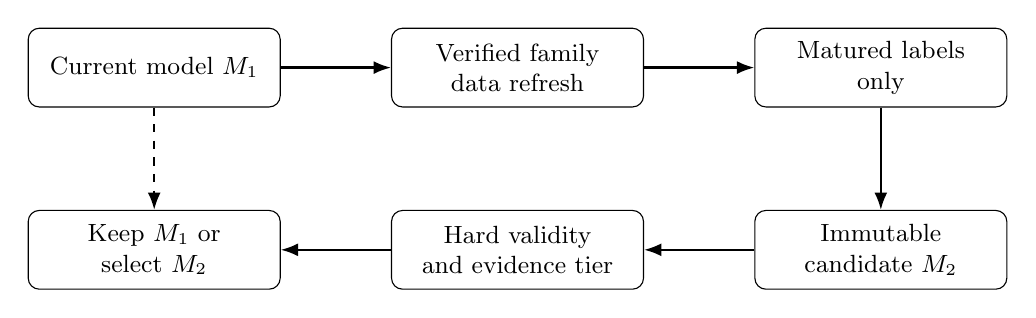
\begin{tikzpicture}[
  font=\small,
  box/.style={draw,rounded corners,align=center,minimum width=32mm,minimum height=10mm,inner sep=3pt},
  arr/.style={-{Latex[length=2.2mm]},thick}
]
\node[box] (m1) {Current model $M_1$};
\node[box, right=14mm of m1] (data) {Verified family\\data refresh};
\node[box, right=14mm of data] (mature) {Matured labels\\only};
\node[box, below=13mm of mature] (m2) {Immutable\\candidate $M_2$};
\node[box, below=13mm of data] (eval) {Hard validity\\and evidence tier};
\node[box, below=13mm of m1] (choice) {Keep $M_1$ or\\select $M_2$};
\draw[arr] (m1)--(data);
\draw[arr] (data)--(mature);
\draw[arr] (mature)--(m2);
\draw[arr] (m2)--(eval);
\draw[arr] (eval)--(choice);
\draw[arr,dashed] (m1)--(choice);
\end{tikzpicture}
\caption{Maintenance never overwrites $M_1$. The dashed path is the product safety property: Forecast stays available while a candidate is trained, rejected or not ready.}
\end{figure}

The dashed path is important: maintenance must not destroy the current model. If the candidate is invalid, weak, interrupted or not ready, the current artifact remains available. A stronger candidate can be selected explicitly after comparison.

\section{Why Model Update and Forecast Must be Decoupled}
A product can become unusable if a maintenance recommendation is treated as a prerequisite for inference. Consider a pooled model trained through 2022 and a new ticker with current prices through 2026. The ticker can provide today's feature vector even though the family model is old. If the planner interprets the ticker's current date as proof that the family model is stale and forces an update before Forecast, a retraining defect can block an otherwise valid probability.

The correct design separates two statements:
\begin{enumerate}[itemsep=0.2em]
\item ``A forecast can be produced from the current hard-valid model.''
\item ``A newer family model should be investigated because additional matured training evidence exists.''
\end{enumerate}
Both can be true simultaneously.

\section{Scientific Interpretation of the Reference Results}
The reference tables in this paper should be read as examples of evidence classification rather than a contest to maximize AUC.

The Bayesian reference models show that a coherent model can have limited predictive value. Their existence is useful because they provide a stable reference and because they prevent the product from interpreting a weak test result as a software failure. At the same time, the negative or near-zero skill values are a warning against overstating the probabilities.

The regime-aware results show that additional structure does not guarantee improvement. The 24-month regime model improves selected proper scores in the reference sample, but the broader calibration and ranking evidence remains insufficient for promotion. This is precisely the behavior desired from the model ladder: complexity is visible and testable without being automatically trusted.

The enhanced twelve-month result shows a modest improvement under the current research gate. Its role is not to prove that machine learning predicts markets reliably; its role is to demonstrate that the architecture can prefer a stronger exact-domain model when the evidence supports it.

\section{Reproducibility Checklist for an External Reviewer}
An independent reviewer should be able to reconstruct the following chain:
\begin{enumerate}[itemsep=0.2em]
\item identify the exact model manifest;
\item verify the serialized artifact hash;
\item identify the target, benchmark, horizon and hurdle;
\item identify the training universe and date span;
\item inspect data-quality limitations;
\item reproduce the feature contract;
\item confirm that labels mature after the observation date;
\item reproduce chronological split boundaries;
\item verify that the locked test was not used for fitting;
\item recompute proper scores and calibration metrics;
\item confirm the evidence tier from the declared thresholds;
\item apply the model to a supported ticker and reproduce the current feature vector;
\item verify that an unsupported domain fails closed;
\item verify that model maintenance produces a new immutable candidate rather than overwriting the current model;
\item verify that baseline Live is tracking-only while stronger tiers require the adaptive gate.
\end{enumerate}

A result that cannot be traced through this chain should not be treated as a reproducible forecast claim.

\section{Conclusion}
A probabilistic financial research system should not force a false choice between scientific caution and product usability. The appropriate solution is to separate validity from evidence strength. Hard-invalid models remain blocked. Hard-valid Bayesian references can provide explicitly limited probabilities. Stronger models must earn stronger claims under protected temporal validation. Live adaptation is a separate governed layer whose parameters update only after delayed outcomes mature.

This architecture also clarifies the role of deterministic analytics: they support interpretation, scenario analysis and research, but they do not become forecast features merely because they are available. The resulting system is therefore less about finding one universally best algorithm and more about enforcing a transparent chain from data provenance to feature contract, probability model, validation evidence, applicability, model selection, maintenance and Live behavior.

\appendix
\section{Mathematical Reference}
\subsection{Sharpe Ratio}
For periodic excess return $e_t=r_t-r_{f,t}$,
\begin{equation}
SR=\frac{\bar e}{s_e}\sqrt{m}.
\end{equation}

\subsection{Sortino Ratio}
With minimum acceptable return $MAR$ and downside deviation $DD$,
\begin{equation}
Sortino=\frac{R_{ann}-MAR}{DD}.
\end{equation}

\subsection{Portfolio VaRiance}
For weights $w$ and covariance matrix $\Sigma$,
\begin{equation}
\sigma_p^2=w^\top\Sigma w.
\end{equation}

\subsection{Black-Scholes-Merton}
For a European call with continuous dividend yield $q$,
\begin{align}
C &= Se^{-qT}N(d_1)-Ke^{-rT}N(d_2),\\
d_1 &= \frac{\ln(S/K)+(r-q+\tfrac12\sigma^2)T}{\sigma\sqrt{T}},\\
d_2 &= d_1-\sigma\sqrt{T}.
\end{align}

\subsection{Bond Price}
For face value $F$, coupon $C$, yield $y$, frequency $m$, and $n$ periods,
\begin{equation}
P=\sum_{k=1}^{n}\frac{C/m}{(1+y/m)^k}+\frac{F}{(1+y/m)^n}.
\end{equation}

\section{Suggested Model-Manifest Contract}
A retrainable artifact should include a machine-readable block of the form:
\begin{verbatim}
training_contract:
  trainer_family: bayesian_reference
  recipe_id: core-us-12m
  feature_contract: monthly_relative_v1
  benchmark_family: US_LARGE_CAP
  horizon_months: 12
  retrain_supported: true
\end{verbatim}
This prevents runtime retraining logic from inferring scientific behavior from a display name.

\section{Glossary}
\begin{description}[style=nextline]
\item[Anchor] Frozen forecast probability used as the base for Live.
\item[Applicability domain] Declared market, asset-class, security-type, benchmark, horizon and feature conditions under which a model may be used.
\item[Bayesian baseline] Hard-valid Bayesian probability model with limited demonstrated predictive evidence.
\item[Calibration] Agreement between stated probabilities and observed frequencies.
\item[Candidate] Newly trained immutable model not yet selected as current.
\item[Locked test] Final chronological evaluation set excluded from fitting and tuning.
\item[Matured label] Forward outcome whose exact forecast horizon endpoint is now observable.
\item[Proper scoring rule] Loss function whose expected value is optimized by reporting the true probability distribution.
\item[Regime model] Model that introduces a latent market-state representation.
\item[Retraining contract] Explicit manifest declaration describing how an artifact can be rebuilt or updated.
\item[Tracking-only Live] Live workspace using the frozen anchor without adaptive learning or residual application.
\end{description}


\section{Formal Validation Definitions}
This section collects the principal statistical quantities used by the forecast evidence contract.

\subsection{Reference Probability and Brier Skill}
Let $\bar y_{dev}$ be the event rate estimated from the permitted development sample. The reference probability is $p_{ref}=\bar y_{dev}$. For a test set of size $n$,
\begin{align}
BS_{model} &= \frac{1}{n}\sum_{i=1}^n(p_i-y_i)^2,\\
BS_{ref} &= \frac{1}{n}\sum_{i=1}^n(p_{ref}-y_i)^2,\\
BSS &= 1-\frac{BS_{model}}{BS_{ref}}.
\end{align}
Positive Brier skill indicates improvement over the reference probability on that sample. Negative skill indicates worse probability error than the reference. A small positive value should not be interpreted as economically large without uncertainty analysis.

\subsection{Log-Loss Skill}
With mean log losses $LL_{model}$ and $LL_{ref}$,
\begin{equation}
LLS=1-\frac{LL_{model}}{LL_{ref}}.
\end{equation}
Because log loss strongly penalizes confident mistakes, it is useful for detecting models that appear directionally informative but are too aggressive in their probabilities.

\subsection{Expected Calibration Error}
Partition predictions into bins $B_k$. If $\operatorname{conf}(B_k)$ is the mean forecast probability and $\operatorname{acc}(B_k)$ the observed event rate,
\begin{equation}
ECE=\sum_k\frac{|B_k|}{n}\left|\operatorname{acc}(B_k)-\operatorname{conf}(B_k)\right|.
\end{equation}
ECE is easy to understand but depends on binning. It is therefore interpreted alongside calibration slope/intercept and proper scores.

\subsection{Calibration Slope and Intercept}
A diagnostic logistic regression can relate the outcome to the logit of the forecast probability. Ideal calibration corresponds approximately to intercept zero and slope one. A slope below one often indicates over-dispersion or overconfidence; a negative slope is a severe warning that forecast ordering and outcome direction are inconsistent in the evaluation sample.

\subsection{Average Precision and Class Imbalance}
When the event rate differs substantially from 0.5, average precision can supplement ROC AUC because it emphasizes positive-class retrieval. Its baseline depends on event prevalence. It should not replace proper scoring rules for probability assessment.

\section{Hard-Validity Checklist}
The following conditions are treated as model-existence conditions rather than predictive-skill conditions.
\begin{longtable}{p{0.30\textwidth}p{0.62\textwidth}}
\toprule
Check & Rationale\\
\midrule
\endhead
Chronological ordering & Training information must precede evaluation information.\\
Target maturity & Every supervised label must have an observable horizon endpoint.\\
Target-end purge & Earlier fitting rows cannot use outcomes crossing a later evaluation boundary.\\
Embargo & A temporal gap reduces dependence leakage around partition boundaries.\\
Both classes & Binary probability estimation is not meaningful if one outcome class is absent.\\
Minimum rows/dates/span & A large row count concentrated on a few dates is not sufficient temporal evidence.\\
Finite parameters & NaN or infinite coefficients indicate an invalid numerical fit.\\
Finite posterior covariance & Uncertainty propagation requires a usable covariance approximation.\\
Valid probability range & Forecasts must be finite and strictly bounded as required by the implementation.\\
Feature completeness & Runtime features must match the trained feature contract.\\
Benchmark alignment & The event definition depends on the correct benchmark family.\\
Applicability match & Market, asset class, security type and horizon must be within the declared domain.\\
Provenance presence & The model must identify the source corpus and training-period boundaries.\\
\bottomrule
\end{longtable}

\section{Feature Dictionary for the Reference Family}
The reference feature family is intentionally small enough to audit. The exact implementation contract is versioned, but the following classes capture the intended semantics.
\begin{longtable}{p{0.26\textwidth}p{0.64\textwidth}}
\toprule
Feature class & Interpretation\\
\midrule
\endhead
Relative 1-month return & Recent security return minus benchmark return.\\
Relative 3-month return & Medium-short relative momentum.\\
Relative 6-month return & Medium-horizon relative momentum.\\
Relative 12-month return & Longer relative momentum / reversal context.\\
Security volatility & Realized volatility from past security returns only.\\
Benchmark volatility & Market-regime intensity from benchmark returns.\\
Drawdown & Distance below a trailing security price peak.\\
Trend distance & Relationship between short and long moving trends.\\
Downside volatility & Realized dispersion of negative returns.\\
Correlation & Historical security-benchmark co-movement.\\
Rolling beta & Historical sensitivity to benchmark moves.\\
Regime probabilities & Filtered probabilities of latent benchmark market states.\\
\bottomrule
\end{longtable}

A feature is not accepted merely because it has an intuitive story. The feature must have a point-in-time definition, reproducible computation, missing-data policy and protected evaluation record.

\section{Training, Validation and Inference Lifecycle}
The lifecycle can be represented as a sequence of immutable evidence states.
\begin{enumerate}[itemsep=0.2em]
\item \textbf{Acquire or refresh data.} Update the durable research store independently of model fitting.
\item \textbf{Assess readiness.} Verify benchmark coverage, target coverage and horizon-dependent history.
\item \textbf{Freeze dataset.} Build backward-looking features and matured targets, then write hashes and split metadata.
\item \textbf{Train.} Fit the declared trainer family using development data only.
\item \textbf{Calibrate.} Use the dedicated validation partition or stage.
\item \textbf{Evaluate locked test.} Compute proper scores, ranking, calibration and temporal diagnostics.
\item \textbf{Classify evidence.} Distinguish hard-invalid, baseline, validated research and validated market.
\item \textbf{Save immutable candidate.} Persist model, manifest, evidence and lineage.
\item \textbf{Select explicitly.} Do not replace the current stronger model automatically.
\item \textbf{Serve inference.} Resolve the model by applicability and horizon, verify artifact integrity, construct current features and produce the probability.
\end{enumerate}

The important design property is that data acquisition, training, validation, model selection and Live adaptation are separable operations. A failure in one stage does not silently mutate another.

\section{Runtime Retraining Contracts}
A clean runtime system requires more than a saved model file. Every retrainable artifact must declare how it is to be rebuilt. The retraining contract is conceptually distinct from a display profile. It contains at least:
\begin{itemize}[itemsep=0.15em]
\item trainer family;
\item recipe identifier;
\item horizon;
\item benchmark family;
\item feature contract;
\item data-frequency convention;
\item minimum required history;
\item retrain-support flag;
\item promotion rules.
\end{itemize}

This prevents a common integration error in which a model profile such as ``Bayesian reference 12 month'' is mistakenly treated as the ID of a training recipe. Human-readable names are presentation metadata; they are not scientific execution contracts.

\section{Guided Planner as a Capability Model}
A single field called \texttt{recommended\_action} is insufficient when maintenance can fail independently of inference. A more robust planner separates capabilities from recommendations.
\begin{verbatim}
can_forecast_now: true
can_start_live_now: true
live_mode: tracking_only
instrument_data_update_available: false
model_update_available: true
model_update_required: false
recommended_action: forecast
\end{verbatim}
This structure allows the UI to show a forecast immediately while still advising the user that the family model is aging. It also permits a failed optional update to fall back cleanly to the current model.

\section{New-Ticker Pooled-Family Semantics}
A pooled model estimates a relationship learned across a training universe. When a new ticker is entered, there are two conceptually different datasets:
\begin{enumerate}[itemsep=0.2em]
\item the historical family corpus used to fit the model;
\item the new ticker's recent history used to calculate today's feature vector.
\end{enumerate}
The new ticker need not become part of the training corpus before the model can be applied. What matters is that the ticker lies within the declared applicability domain and that its current feature vector can be constructed under the same contract.

This distinction is essential to usability. If every new ticker forced a retrain, the product would collapse back into a per-ticker laboratory rather than a forecasting application.

\section{Live State and Delayed-Outcome Data Model}
A pending Live observation should retain enough information to resolve the future event exactly and update only the state lineage that produced it. A minimal record includes:
\begin{itemize}[itemsep=0.15em]
\item unique pending-label ID;
\item ticker and benchmark;
\item base model ID;
\item adaptive settings fingerprint;
\item observation timestamp and date;
\item entry prices;
\item horizon and hurdle;
\item anchor probability;
\item candidate probability;
\item adaptive feature vector;
\item earliest maturity date.
\end{itemize}

When the horizon matures, the outcome is computed from the exact common-session endpoint. The prediction is scored before the adaptive posterior is updated. This preserves a genuine out-of-sample sequence.

\section{Analytical Result Contract}
A deterministic analytical number should not be returned as an unexplained float when provenance matters. A robust result object contains:
\begin{verbatim}
metric
value
display
formula_id
period
as_of
inputs
source_refs
quality_flags
method_version
\end{verbatim}
This contract makes it possible to distinguish, for example, a ratio calculated from reported values from one containing a derived denominator, or a DCF built from one currency from a valuation that would otherwise mix currencies.

\section{Normalized Statement Semantics}
Financial statement normalization requires explicit accounting semantics. Provider aliases should map into canonical fields such as revenue, gross profit, operating income, taxes, D\&A, capital expenditure, working capital, debt, cash and diluted shares. A normalized value should carry status such as reported, mapped, derived, unavailable or not applicable.

Derived identities must be conservative. For example, free cash flow can be derived from operating cash flow and capital expenditure when both are available, but a missing capex field must not be interpreted as zero. Similarly, total debt can be derived from short- and long-term components when the provider supplies them, but missing debt concepts should remain missing.

\section{DCF Methodology in Greater Detail}
The DCF module deliberately separates historical statement normalization from forward assumptions. Historical inputs are evidence. Forward growth, margins, WACC and terminal assumptions are scenarios.

For projection year $t$,
\begin{align}
Revenue_t &= Revenue_{t-1}(1+g_t),\\
EBIT_t &= Revenue_t\cdot m_t,\\
NOPAT_t &= EBIT_t(1-T_t),\\
FCFF_t &= NOPAT_t+D\&A_t-CapEx_t-\Delta NWC_t.
\end{align}
A perpetual-growth terminal value is
\begin{equation}
TV_N=\frac{FCFF_{N+1}}{WACC-g},\qquad g<WACC.
\end{equation}
An exit-multiple terminal value uses a selected operating metric multiplied by a terminal multiple. Enterprise value is bridged to equity value by adding cash-like assets and subtracting net debt or equivalent claims under the chosen convention, then dividing by diluted shares for a per-share estimate.

The tool should reject structurally invalid assumptions such as $g\ge WACC$ rather than returning a mathematically explosive valuation.

\section{Options Methodology in Greater Detail}
Black-Scholes-Merton assumes lognormal diffusion, continuous trading, frictionless markets, known rates/volatility under the model, and European exercise. The formula is useful as a theoretical benchmark, not a complete model of listed-option markets.

The Greeks are local derivatives of the pricing equation. Gamma and Vega can become large near particular moneyness and expiry conditions. Theta is convention-sensitive and should state whether it is reported per year or converted to a daily basis. Implied volatility is recovered numerically by inverting the pricing function and must fail safely when the market price lies outside the bracketable theoretical range.

\section{Factor-Model Methodology in Greater Detail}
For design matrix $X$ and return vector $y$, OLS estimates
\begin{equation}
\hat\beta=(X^\top X)^{-1}X^\top y
\end{equation}
when the design has full rank. Standard errors depend on the residual variance model. The current descriptive factor layer is not a causal inference engine and does not convert a statistically significant exposure into a forecast feature automatically.

Rolling beta is similarly descriptive. Window length, return frequency and benchmark choice materially affect the estimate. Users should interpret rolling beta as a changing historical exposure rather than an intrinsic constant property of the security.

\section{Release Acceptance Matrix}
A release claiming a complete forecasting workflow should demonstrate at least the following behavioral matrix.
\begin{longtable}{p{0.35\textwidth}p{0.55\textwidth}}
\toprule
Scenario & Required outcome\\
\midrule
\endhead
New supported US common stock & Data resolves, pooled family selected, Forecast produced.\\
Missing local price history & Update data, replan automatically, Forecast produced when sufficient.\\
Baseline-only horizon & Forecast produced with Limited evidence; Start Live enters tracking-only mode.\\
Validated-model horizon & Stronger model preferred; adaptive Live eligible after explicit activation and gate checks.\\
Model aging & Forecast remains available; maintenance shown as a separate recommendation.\\
Optional retrain not ready & Current Forecast remains available.\\
Optional retrain fails computationally & Current Forecast remains available.\\
Optional retrain lacks stronger evidence & Candidate retained appropriately; current stronger model not silently downgraded.\\
Unsupported asset class & Analytics may run; Forecast blocked with plain explanation.\\
Application restart & Local corpus, model registry and coherent user state persist.\\
\bottomrule
\end{longtable}

\section{Testing Philosophy}
A large unit-test count is not sufficient evidence for an end-to-end product. Source-string tests can prove that a button or endpoint name exists while missing an integration defect between the button, endpoint, manifest and trainer.

The release test pyramid should therefore include:
\begin{enumerate}[itemsep=0.2em]
\item formula-level known-answer tests;
\item data-integrity and leakage tests;
\item model-validity and evidence-tier tests;
\item API integration tests using actual bundled model IDs;
\item failure-path tests;
\item clean-directory application tests;
\item packaged executable new-ticker Forecast/Live smoke tests;
\item restart persistence tests.
\end{enumerate}


\section{What the Public Repository Implements}
The public tree at \texttt{github.com/rajeevyadav/fincompass} (application \texttt{VERSION} 2.0.0) already contains the layers described in this paper. It is important to separate \emph{implemented} from \emph{empirically strong}.

Implemented today:
\begin{itemize}[itemsep=0.15em]
\item evidence engine, instrument classification and benchmark resolution;
\item durable local research store with overlap/tail refresh;
\item backward-looking price features and optional SEC fundamental features;
\item Bayesian reference artifacts at 6, 12, 24 and 36 months;
\item regime-aware Bayesian artifacts as research alternatives;
\item one 12-month enhanced ensemble at the research-validated tier;
\item chronological purge/embargo, calibration, proper scores and block bootstrap;
\item Live residual with delayed labels and a prequential gate;
\item a deterministic analytics library that is not automatically a feature source.
\end{itemize}

Not yet closed as a product path, and therefore not a modelling problem first:
\begin{itemize}[itemsep=0.15em]
\item pooled-model freshness still risk being judged against the arbitrary target ticker;
\item runtime retraining still risks inferring a recipe from a display profile;
\item Model Lab recipes exist for 6-month and 12-month families, not for 24-month or 36-month retraining;
\item Guided Start Live can still attempt baseline activation even though tracking-only Live exists in the backend.
\end{itemize}

The bundled locked-test tables should be read against that inventory. They demonstrate the tier machinery on a small surviving-name sample. They do not establish market-grade skill.

\section{Path to Stronger Model Performance}
Better performance will not come from replacing the Bayesian reference with a larger network on eight names. It comes from a larger honest sample, a tighter feature contract, and a model that must still beat the reference on proper scores.

The working order is fixed.

\paragraph{Close the user path first.}
A new supported ticker must reach Forecast and Live without Model Lab. An optional update failure must leave the current Forecast standing. Until that is true, additional model families only multiply dead ends.

\paragraph{Enlarge the training universe before the algorithm.}
A 12-month relative-return classifier needs hundreds of names, including later delistings, and point-in-time membership of the benchmark family. Monthly rows on eight survivors overstate independence.

\paragraph{Freeze one target.}
Optimize first
\[
Y=\I\!\left[R_{i,t}^{(12)}-R_{\mathrm{SPX},t}^{(12)}>0\right]
\]
at month-end frequency. Other horizons and benchmarks are separate families.

\paragraph{Admit features only with provenance.}
The coded optional SEC features --- revenue growth, margins, leverage, free-cash-flow margin, ROA --- are the first candidates, merged on filing date. Technical indicators that already exist in the analytics library stay out of Forecast unless they survive an ablation on development data and a single locked-test read.

\paragraph{Keep the ladder.}
Every new corpus trains (1) the unconditional rate, (2) the Bayesian reference and (3) the enhanced ensemble on the same split. A new algorithm is added only after (3) beats (2) on Brier skill, log-loss skill, ECE and walk-forward sign, not on AUC alone.

\paragraph{Tighten gates only after the sample is real.}
The current research floor (\texttt{min\_auc} 0.50, \texttt{min\_brier\_skill} $-0.02$) is appropriate for a small demonstration corpus. On a larger corpus a Guided-default 12-month model should be required to show positive proper-score skill, a bootstrap lower bound near zero or better, multi-year walk-forward stability and an ECE small enough to read the number as a probability.

\paragraph{Live last.}
Adaptive skill is measured against the frozen anchor, not against the event rate. If the residual loses, the residual stays at zero.

A companion playbook in the documentation package lists the 90-day sequence, the experiment log template and the repository files to touch.

\section{Research Extensions}
Several extensions are scientifically interesting but should remain secondary to a reliable baseline workflow.

\subsection{Hierarchical Market-Family Models}
A hierarchical Bayesian model could partially pool coefficients across regions, sectors or capitalization groups while preserving domain-specific deviations. This may improve data efficiency, but only if cross-market currency, calendar and benchmark semantics are handled explicitly.

\subsection{Dynamic Coefficients}
State-space or dynamic logistic models can allow coefficients to evolve over time. These approaches are attractive under nonstationarity but add process-noise choices and can increase uncertainty. They should be judged against the fixed-coefficient Bayesian reference.

\subsection{Bayesian Model Averaging}
Rather than selecting one complex model, posterior or evidence-weighted model averaging could combine structurally different candidates. Such weighting must be trained inside development data and must not use the locked test.

\subsection{Point-in-Time Factor and Macro Features}
Broader fundamentals and macro variables can be added only when publication-time semantics are robust. Historical revised macro series or restated statements can create subtle hindsight bias if treated as contemporaneously available.

\subsection{Cross-Sectional Portfolio Forecasting}
A future portfolio layer could model joint relative-return probabilities rather than averaging individual probabilities. This would require explicit dependence modeling, portfolio constraints and a separate validation target.

\bibliographystyle{plainnat}
\bibliography{refs}
\end{document}
